\documentclass[12pt]{article}



%%%%%%%%%%%%%%%%%%%%%%%%%%%%%%%%%%%%%%
% Metainformation
%%%%%%%%%%%%%%%%%%%%%%%%%%%%%%%%%%%%%%
\newcommand{\trauthor}{Leopold Lemmermann}
\newcommand{\trtype}{Paper}
\newcommand{\trtitle}{Image Captioning}
\newcommand{\trdate}{\today}



%%%%%%%%%%%%%%%%%%%%%%%%%%%%%%%%%%%%%%
% Language
%%%%%%%%%%%%%%%%%%%%%%%%%%%%%%%%%%%%%%
\usepackage[english]{babel}
\selectlanguage{english}



%%%%%%%%%%%%%%%%%%%%%%%%%%%%%%%%%%%%%%
% Bind packages
%%%%%%%%%%%%%%%%%%%%%%%%%%%%%%%%%%%%%%
\usepackage{acronym}                    % Acronyms
\usepackage{algorithmic}                % Algorithms and Pseudocode
\usepackage{algorithm}                  % Algorithms and Pseudocode
\usepackage{amsfonts}                   % AMS Math Packet (Fonts)
\usepackage{amsmath}                    % AMS Math Packet
\usepackage{amssymb}                    % Additional mathematical symbols
\usepackage{amsthm}
\usepackage{booktabs}                   % Nicer tables
% \usepackage[font=small,labelfont=bf]{caption} % Numbered captions for figures
\usepackage{color}                      % Enables defining of colors via \definecolor
\definecolor{uhhRed}{RGB}{254,0,0}      % Official Uni Hamburg Red
\definecolor{uhhGrey}{RGB}{122,122,120} % Official Uni Hamburg Grey
\usepackage{fancybox}                   % Gleichungen einrahmen
\usepackage{fancyhdr}                   % Packet for nicer headers

%\usepackage[outer=3.35cm]{geometry}    % Type area (size, margins...) !!!Release version
%\usepackage[outer=2.5cm]{geometry}     % Type area (size, margins...) !!!Print version
%\usepackage{geometry}                  % Type area (size, margins) !!!Proofread version
\usepackage[outer=3.15cm]{geometry}     % Type area (size, margins...) !!!Draft version
\geometry{a4paper,body={5.8in,9in}}

\usepackage{graphicx}                   % Inclusion of graphics
%\usepackage{latexsym}                  % Special symbols
\usepackage{longtable}                  % Allow tables over several pages
\usepackage{listings}                   % Nicer source code listings
\usepackage{multicol}                   % Content of a table over several columns
\usepackage{multirow}                   % Content of a table over several rows
\usepackage{rotating}                   % Alows to rotate text and objects
\usepackage[hang]{subfigure}            % Allows to use multiple (partial) figures in a fig
%\usepackage[font=footnotesize,labelfont=rm]{subfig}  % Pictures in a floating environment
\usepackage{tabularx}                   % Tables with fixed width but variable rows
\usepackage{url,xspace,boxedminipage}   % Accurate display of URLs



%%%%%%%%%%%%%%%%%%%%%%%%%%%%%%%%%%%%%%
% Configuration
%%%%%%%%%%%%%%%%%%%%%%%%%%%%%%%%%%%%%%
\hyphenation{whe-ther}                  % Manually use: "\-" in a word: Staats\-ver\-trag

%\lstloadlanguages{C}                   % Set the default language for listings
\DeclareGraphicsExtensions{.pdf,.svg,.jpg,.png,.eps} % first try pdf, then eps, png and jpg
\graphicspath{{./src/}}                 % Path to a folder where all pictures are located
\pagestyle{fancy}                       % Use nicer header and footer

% Redefine the environments for floating objects:
\setcounter{topnumber}{3}
\setcounter{bottomnumber}{2}
\setcounter{totalnumber}{4}
\renewcommand{\topfraction}{0.9}        %Standard: 0.7
\renewcommand{\bottomfraction}{0.5}     %Standard: 0.3
\renewcommand{\textfraction}{0.1}       %Standard: 0.2
\renewcommand{\floatpagefraction}{0.8}  %Standard: 0.5

% Tables with a nicer padding:
\renewcommand{\arraystretch}{1.2}



%%%%%%%%%%%%%%%%%%%%%%%%%%%%%%%%%%%%%%
% Additional 'theorem' and 'definition' blocks
%%%%%%%%%%%%%%%%%%%%%%%%%%%%%%%%%%%%%%
\theoremstyle{plain}
\newtheorem{theorem}{Theorem}[section]
\newtheorem{axiom}{Axiom}[section]
%Usage:%\begin{axiom}[optional description]%Main part%\end{fakt}

\theoremstyle{definition}
\newtheorem{definition}{Definition}[section]

%Additional types of axioms:
\newtheorem{lemma}[axiom]{Lemma}
\newtheorem{observation}[axiom]{Observation}

%Additional types of definitions:
\theoremstyle{remark}
\newtheorem{remark}[definition]{Remark}



%%%%%%%%%%%%%%%%%%%%%%%%%%%%%%%%%%%%%%
% Abbreviations and mathematical symbols
%%%%%%%%%%%%%%%%%%%%%%%%%%%%%%%%%%%%%%
\newcommand{\modd}{\text{ mod }}
\newcommand{\RS}{\mathbb{R}}
\newcommand{\NS}{\mathbb{N}}
\newcommand{\ZS}{\mathbb{Z}}
\newcommand{\dnormal}{\mathit{N}}
\newcommand{\duniform}{\mathit{U}}

\newcommand{\erdos}{Erd\H{o}s}
\newcommand{\renyi}{-R\'{e}nyi}



%%%%%%%%%%%%%%%%%%%%%%%%%%%%%%%%%%%%%%
% Document:
%%%%%%%%%%%%%%%%%%%%%%%%%%%%%%%%%%%%%%
\begin{document}
\renewcommand{\headheight}{14.5pt}

\fancyhead{}
\fancyhead[CO]{\trtitle}



%%%%%%%%%%%%%%%%%%%%%%%%%%%%%%%%%%%%%%
% Cover
%%%%%%%%%%%%%%%%%%%%%%%%%%%%%%%%%%%%%%
\title{\trtitle\\[0.2cm]{\normalsize\trtype}}
\author{\trauthor}
\date{\trdate}
\maketitle

\thispagestyle{empty}

\begin{center}
    \includegraphics[width=0.2\textwidth]{res/wtmicon.pdf}
\end{center}

\begin{abstract}
 This paper is about image captioning. We discuss the current state of the art and overview the most important methods. We present the results of our experiments with different encoder and decoder models. We use the flickr8k dataset and evaluate the models using the BLEU score. We discuss the results and give an outlook on future work.
\end{abstract}

\tableofcontents
\newpage
\pagenumbering{arabic}



%%%%%%%%%%%%%%%%%%%%%%%%%%%%%%%%%%%%%%
% Content
%%%%%%%%%%%%%%%%%%%%%%%%%%%%%%%%%%%%%%
\section{Introduction}
\label{sec:introduction}

Image captioning involves generating textual descriptions of given images. It is a complex problem because it combines the visual and textual domains. In recent years, deep learning has revolutionized the field of image captioning.

Image captioning is a complex and interdisciplinary task bridging computer vision (CV) and natural language processing (NLP). Generating natural, descriptive sentences for images involves detecting and interpreting visual elements and their relationships within depicted scenes. Recent advancements leverage deep learning, particularly Convolutional Neural Networks (CNNs) for feature extraction and Recurrent Neural Networks (RNNs) for sequential language generation. For instance, models such as "Show and Tell" \cite{Vinyals:2015} and "Show, Attend, and Tell" \cite{Xu} utilize CNN-RNN architectures, with the latter integrating attention mechanisms to enhance focus on specific image regions, thereby improving caption relevance and accuracy.

Additionally, methods like Reinforcement Learning (RL) have been explored to optimize these models directly on evaluation metrics, addressing issues such as exposure bias by aligning training and inference methods more closely \cite{Rennie}.

Another approach has dealt with the tendency of beam search to produce near-duplicate captions. Diverse Beam Search ensures that generated captions capture a broader range of plausible descriptions, reflecting the inherent ambiguity in image captioning tasks \cite{Vijayakumar}.

We begin by discussing the most critical methods in image captioning. We then present the results of our experiments with different encoder and decoder models. We use the flickr8k dataset and evaluate the models using the BLEU score. We discuss the results and give an outlook on future work.



\section{Methods}
\label{sec:methods}

In image captioning tasks, a model takes an image as input and generates a caption as output. The model consists of an encoder that extracts features from the image and a decoder that generates the caption. We discuss the dataset, encoder-decoder architecture, encoder models, decoder models, and evaluation metrics.

\subsection{Dataset}
\begin{figure}[H]
    \centering
    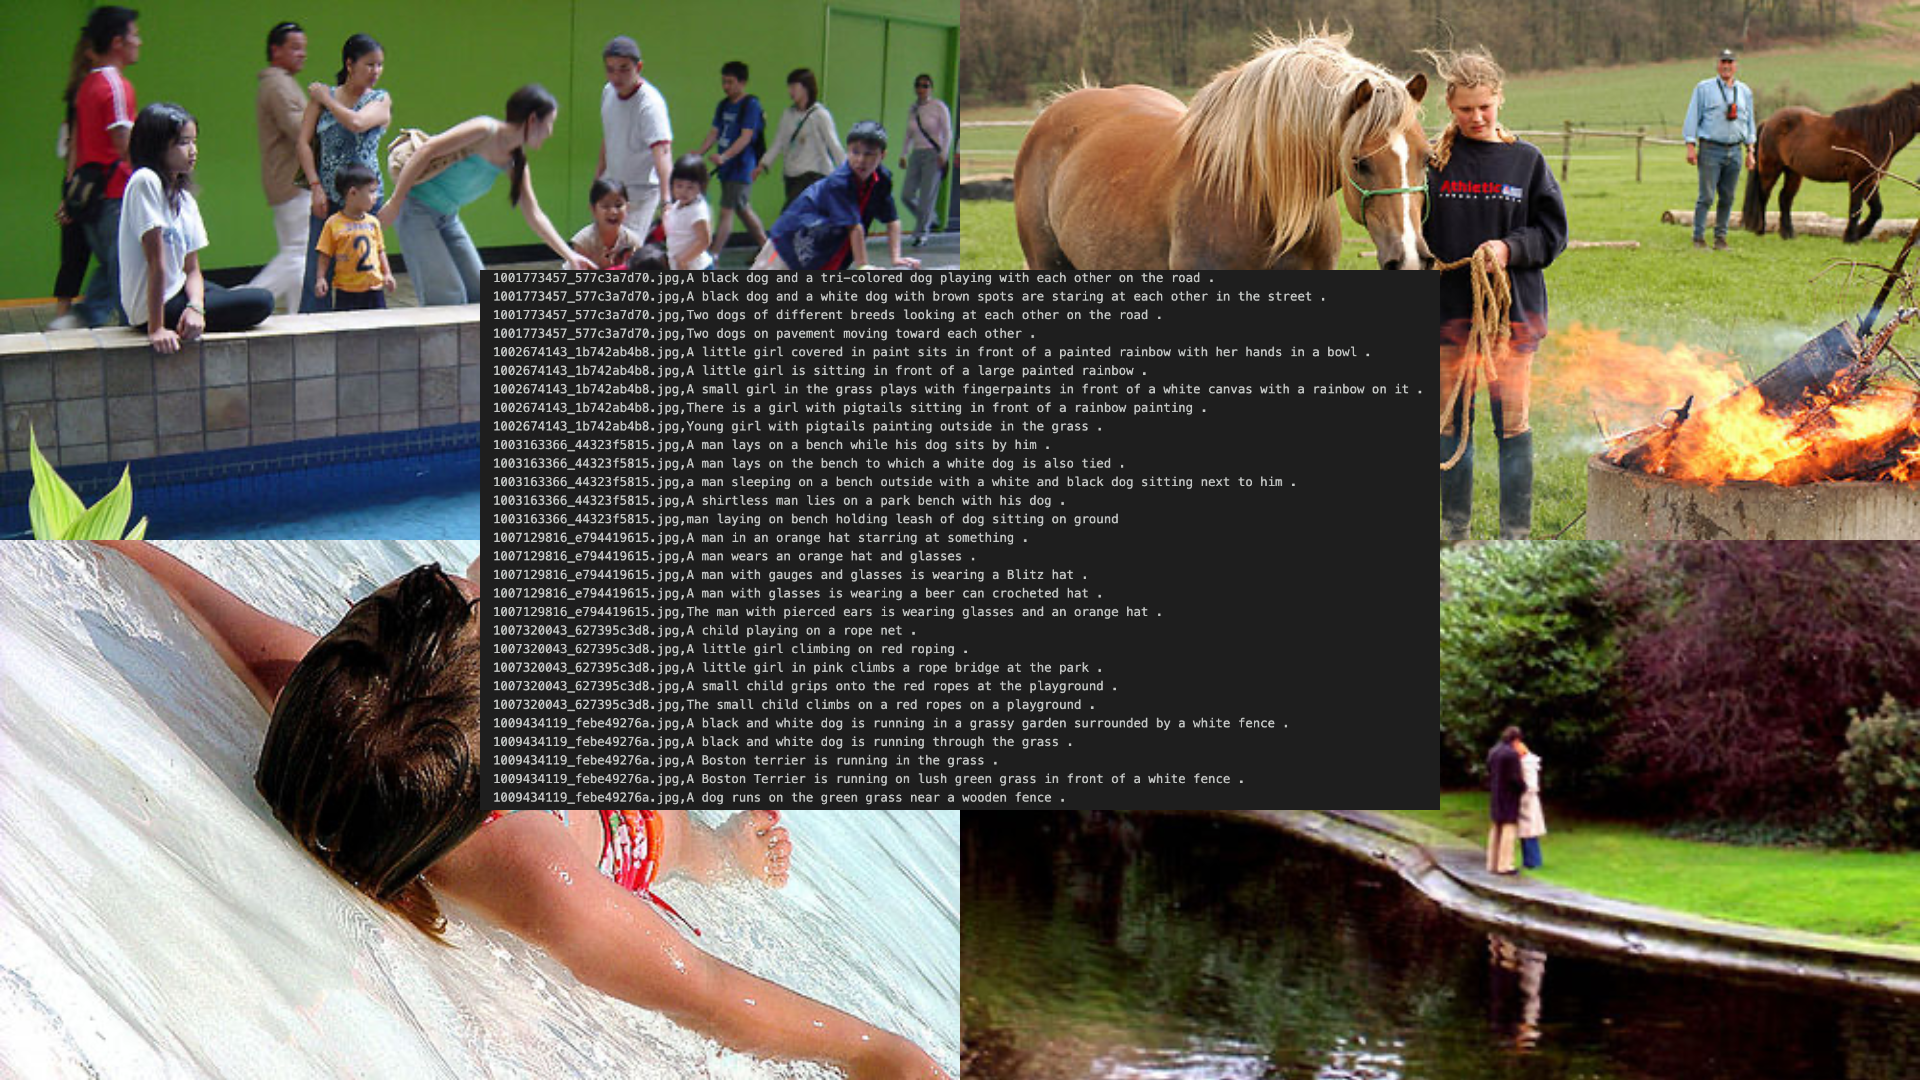
\includegraphics[width=0.7\textwidth]{res/flickr8k.png}
    \caption{Example images and captions from the flickr8k dataset.}
    \label{fig:flickr8k}
\end{figure}
We focused on the flickr8k dataset, a pivotal resource in image captioning. Comprising 8.000 diverse images, each with five reference captions, this dataset is renowned for its quality and is a common choice for image captioning research due to its manageable size.
\par Other commonly used datasets are flickr30k and MS COCO, but these datasets are more extensive and cannot be processed due to our limited computational resources.

\subsection{Encoder-Decoder Architecture}
\begin{figure}[H]
    \centering
    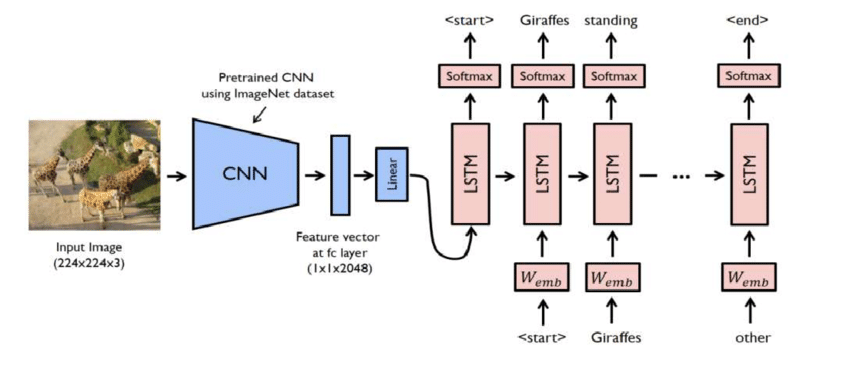
\includegraphics[width=.5\textwidth]{res/encoder-decoder.png}
    \caption{A Survey on Various Deep Learning Models for Automatic Image Captioning \cite{gaurav}}
    \label{fig:encoder-decoder}
\end{figure}
Usually, an encoder-decoder architecture is used to achieve image captioning. The encoder is a convolutional neural network (CNN) that extracts features from the image. The decoder is a recurrent neural network (RNN) that generates the caption word by word.

\subsection{Encoder Models}
We experimented with two different models for encoding images: ResNet-50 and VGG-16.
\par ResNet-50 is a deep residual network widely used for image classification. It has 50 layers and uses skip connections to avoid the vanishing gradient problem. It was introduced in \cite{he}.
VGG-16, a deep convolutional neural network developed by the Visual Geometry Group at the University of Oxford, is known for its simplicity and effectiveness, making it an accessible choice for our research.
Thanks to their pre-training on the ImageNet dataset, the models do not need to be trained from scratch, saving valuable time and computational resources.

\subsection{Decoder Models}
We experimented with two different models for decoding captions: GRU and LSTM.
\par Gated Recurrent Units (GRUs) are a type of RNN similar to LSTMs but with fewer parameters. They are easier to train and faster to compute. They were introduced in \cite{cho}.
\par Long Short-Term Memory (LSTM) networks are a type of RNN designed to avoid the vanishing gradient problem. They have a cell state that can store information over long sequences. They were introduced in \cite{hochreiter}.

\subsection{Evaluation Metrics}
The accuracy of image captioning is commonly measured using BLEU or CIDEr scores.
\par BLEU is a precision-based metric that compares n-grams in the generated caption to those in the reference captions. It ranges from 0 to 1, with higher values indicating better performance. It was introduced in \cite{papineni}.
\par CIDEr is a recall-based metric that compares the generated caption to the reference captions using cosine similarity. Ranging from 0 to 1, higher values indicate better performance. It was introduced in \cite{vedantam}.
\par For simplicity, we only use the BLEU score in our experiments.



\section{Approach}
\label{sec:approach}

Our approach begins with data preprocessing, followed by model training and evaluation.

\subsection{Data Preprocessing}
\par We preprocess the images by resizing them to 224x224 pixels, normalizing the pixel values, and encoding them to tensors of the dimension (224, 224, 3).
\par We create a vocabulary of words and map each word to an index.
\par We preprocess the captions by tokenizing them, converting them to lowercase, and padding them to a fixed length. Then, we encode them using the vocabulary and convert them to one-dimensional tensors with a specified max\_length.

\subsection{Model Training}
We only train the decoder model because the encoder models are pre-trained on ImageNet. We use the Adam optimizer and the categorical cross-entropy loss function. We train our model for the specified number of epochs and save the weights with the best BLEU score on the validation set. The model's state is saved after each epoch to resume training if necessary.

\subsection{Model Evaluation}
Evaluation happens after each training epoch. This approach enables us to monitor the model's performance and save the weights with the best BLEU score. We evaluate the model on the test set using the BLEU score and compare it to the validation set's BLEU score to detect overfitting. These scores are also stored after each epoch to analyze the model's performance over time.



\section{Results}
\label{sec:results}

We present the results of our experiments with different encoder and decoder models. \ref{fig:results} shows the BLEU scores of the models on the test set over the epochs. The detailed BLEU score results are shown in \ref{tab:results}.

\begin{figure}[H]
    \centering
    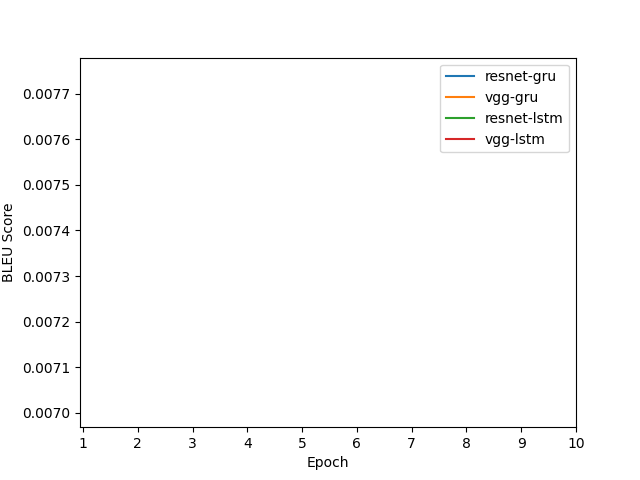
\includegraphics[width=0.8\textwidth]{res/results.png}
    \caption{Results of the experiments with different encoder and decoder models.}
    \label{fig:results}
\end{figure}

\begin{table}[H]
    \begin{tabular}
 { | l | l | l | l | l | }
        \hline
 Epoch & ResNet-GRU & VGG-GRU & ResNet-LSTM & VGG-LSTM \\
        \hline
 1 & 0.0074 & 0.0025 & 0.0035 & 0.0157 \\
 2 & 0.0028 & 0.0024 & 0.0050 & 0.0056 \\
 3 & 0.0024 & 0.0037 & 0.0045 & 0.0055 \\
 4 & 0.0036 & 0.0030 & 0.0034 & 0.0052 \\
 5 & 0.0038 & 0.0025 & 0.0035 & 0.0062 \\
 6 & 0.0056 & 0.0026 & 0.0037 & 0.0069 \\
 7 & 0.0058 & 0.0028 & 0.0038 & 0.0060 \\
 8 & 0.0069 & 0.0031 & 0.0037 & 0.0058 \\
 9 & 0.0045 & 0.0034 & 0.0030 & 0.0058 \\
 10 & 0.0037 & 0.0029 & 0.0034 & 0.0052 \\
        \hline
    \end{tabular}

    \caption{Detailed results of the experiments with different encoder and decoder models.}
    \label{tab:results}
\end{table}

The results show that the VGG encoder with the LSTM decoder achieves the best performance, with a BLEU score of .157 in the first epoch. Other combinations, like the VGG-GRU or the ResNet-LSTM, are significantly worse, with respective BLEU scores of .0025 and .0035 in the first epoch. The ResNet-GRU model performs slightly better, with a BLEU score of .0074 in the first epoch.

For most models, their BLEU score peaks in the first few epochs and then decreases. The VGG-LSTM model is the most stable over the epochs and somewhat contradicts this hypothesis. However, the other models show a similar decrease over the epochs. These findings suggest overfitting to the training data.

Given the mixed nature of the results, it is challenging to draw definitive conclusions. The VGG encoder paired with the LSTM decoder is the most effective combination available., achieving the highest BLEU score in the first epoch. Nevertheless, further experiments are needed to confirm this result.


\section{Conclusion}
\label{sec:conclusion}

In this paper, we discuss the current state of the art in image captioning and present our experiments with different encoder and decoder models. We use the flickr8k dataset and evaluate the models using the BLEU score.

In the future, further experiments could be conducted with
\begin{enumerate}
    \item different encoder and decoder models, like attention mechanisms and transformer models.
    \item different datasets, like flickr30k and MS COCO.
    \item different evaluation metrics, like CIDEr.
\end{enumerate}


%%%%%%%%%%%%%%%%%%%%%%%%%%%%%%%%%%%%%%
% References
%%%%%%%%%%%%%%%%%%%%%%%%%%%%%%%%%%%%%%
\newpage
\thispagestyle{empty}

\bibliographystyle{apalike}
\bibliography{bib}

\end{document}